The goal of this section is to give the necessary information to understand the rest of the thesis. Debugging is a complicated process that is made much harder by distributing the system to more than one physical location. To better understand the methods and principles, this chapter will use a simple example application to comprehend the differences in each method easily.

\section{Flink Framework}
\label{flinkFramework}
The Flink Framework is a stream processing framework for the JVM. It is written in java and scala and can be used with a variety of languages and technologies. As is to be expected the most supported languages are java and scala, although there is also a python wrapper and a few more available. The following section will clarify how exactly a Flink application works and what kind of debugging and logging tools it already has.

\subsection{Basics}
Flink is a Framework for processing applications that are distributed across multiple computers. This part will lay out the foundations of the Flink Framework.
Flink applications have a simple base structure that is used by the developer. Each application defines tasks which have a particular structure. Each task has an input and output stream. These are called source and sink. Because both the source and sink of these tasks are streams, they can be attached to each other thus creating a data flow from task to task until the wanted end state is reached.

\begin{figure}[h!]
    \centering
      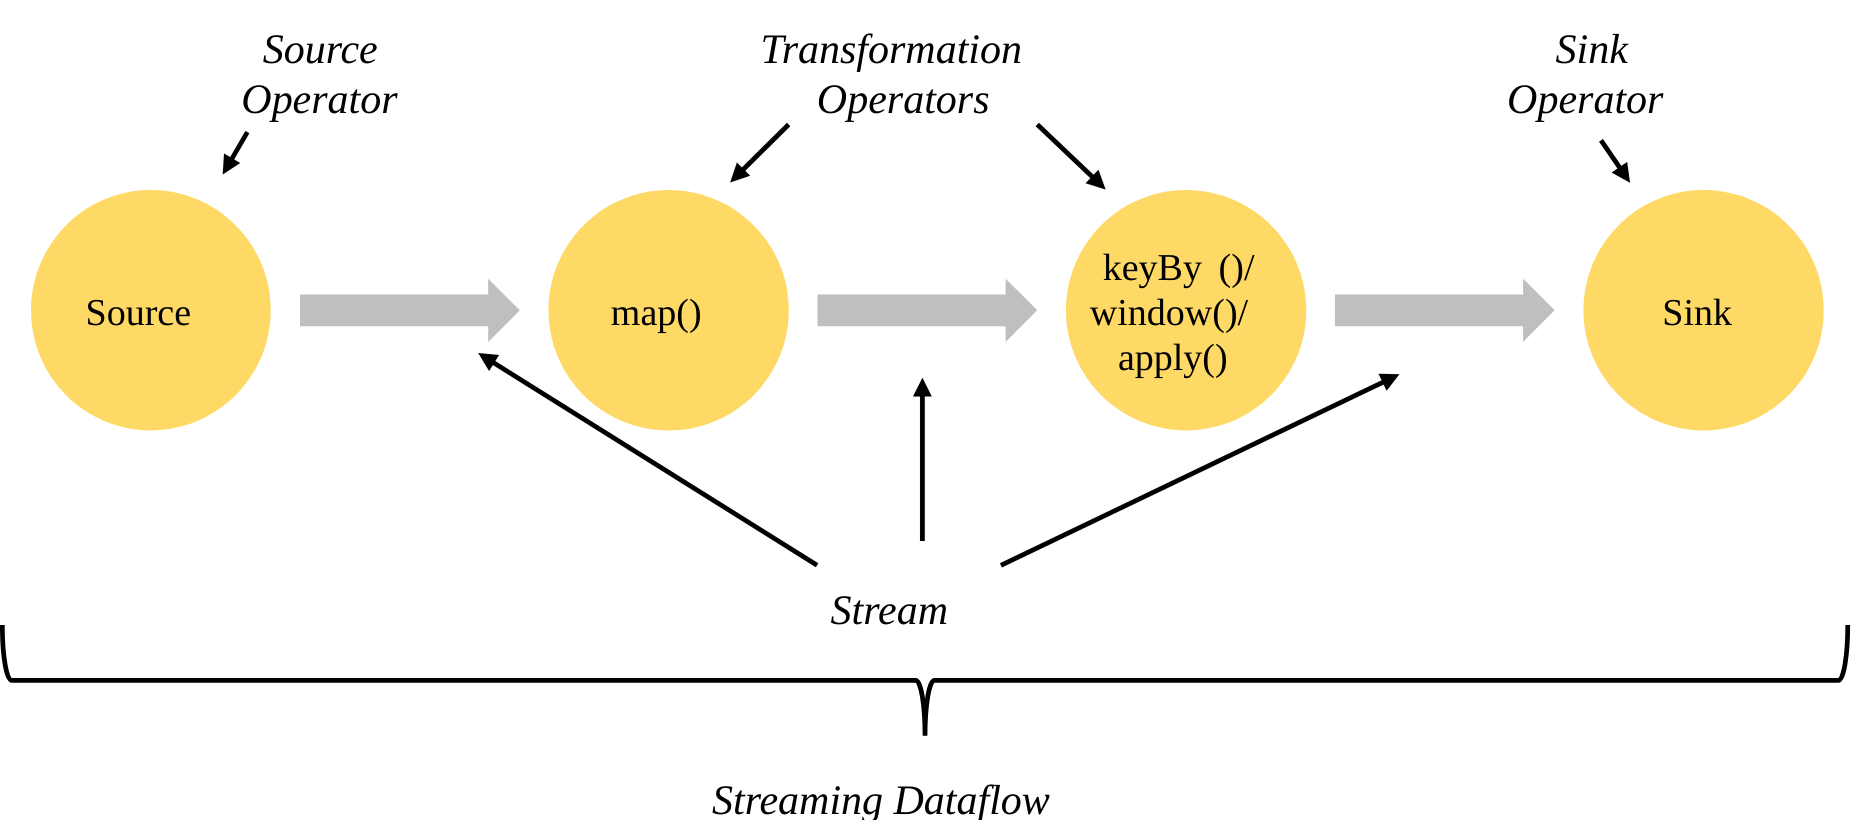
\includegraphics[width=0.9\textwidth]{rw_simpleDataflowInFlink.png}
      \caption{Simple Dataflow in Flink \cite{ApacheFlinkSimpleDataflowFigure}}
      \label{simpleDataflowInFlink}
\end{figure}

Figure \ref{simpleDataflowInFlink} shows a basic program flow. On the left side, it starts with a source. The source is then transferred over a data stream to the first task. The map operation is executed, and the result is sent over a data stream to the next task where the same procedure will start again. The resulting data in this example is the sink, meaning we reached the end of the program. The sink will typically be connected to a database or some other kind of technology for preserving the data. The most basic option would be to write the sink onto the standard output on the console.

Until now the system can only be distributed by having the different tasks on different physical computers. This distribution process will not suffice when the amount of input data gets too high. To achieve real distribution in the application, each task can be run multiple times as so called subtasks. These subtasks run as a single thread in the JVM and are managed by a task manager. Task Managers connect to a Job Manager which coordinates the distributed execution. The data flow from one subtask to another can either be one to one or as a redistributing data flow. A redistributing data flow is necessary to achieve an even distribution of data at the next subtasks.

\begin{figure}[h!]
    \centering
      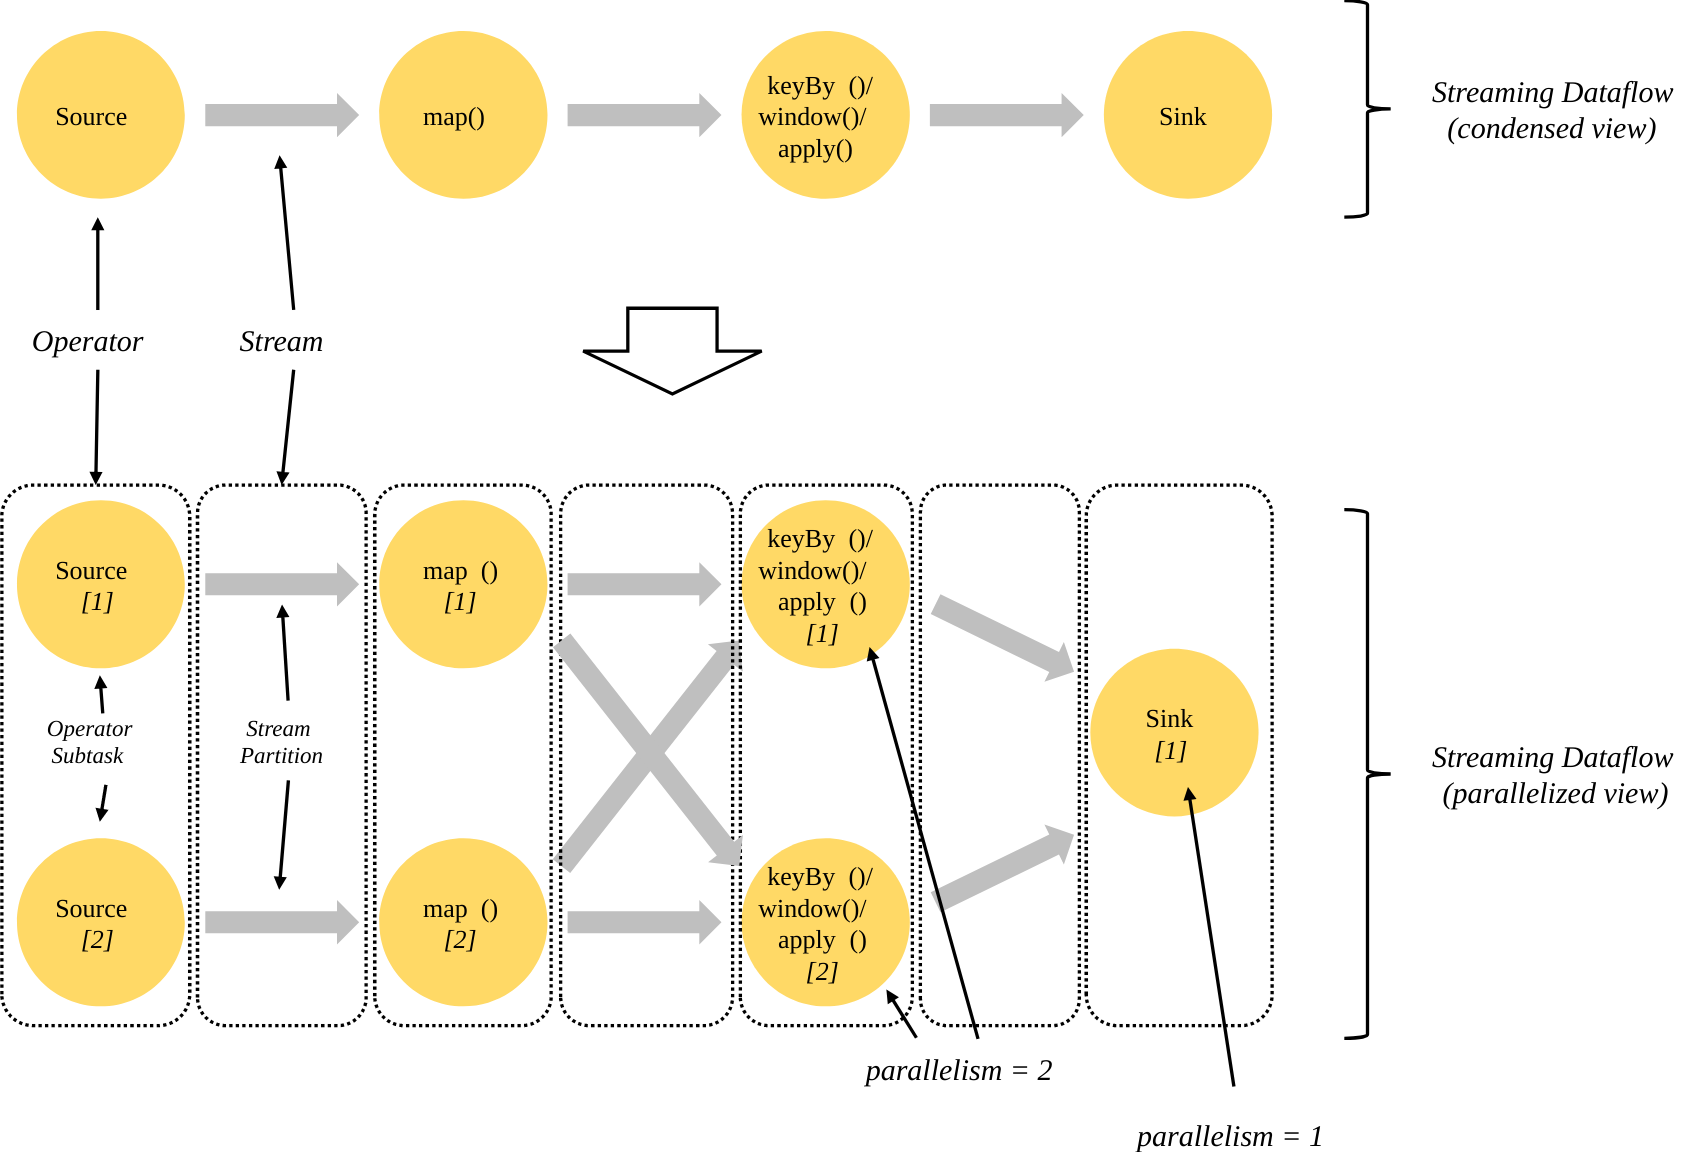
\includegraphics[width=0.9\textwidth]{rw_distributedDataflowInFlink.png}
      \caption{Distributed Dataflow in Flink \cite{ApacheFlinkParallelDataflowFigure}}
      \label{distributedDataflowInFlink}
\end{figure}

Figure \ref{distributedDataflowInFlink} presents the same example as figure \ref{simpleDataflowInFlink} just with the subtasks shown as well. The map task is a vital step in each application as it connects the data from each subtask with each other. It is easily understood by a simple example.
In an application that counts how often each word is in a text, it would only split the text at each space symbol. The redistributing data flow would then create an even distribution in the next node which specifies what to count by (id task) and applies a particular aggregation function to the "apply" operation. The result is then sent to the sink operator. This explanation is a simplification of the actual MapReduce model. For a complete overview see \cite{dean2008mapreduce}.

\subsection{Stream Processing and Batch Processing}

Apache Flink is primarily a stream processing framework, although it can also be used for batch processing. As it makes a big difference in the infrastructure of the framework which process the primary one is, it is important to lay out the differences between the two.

\paragraph{Stream Processing} uses as the name suggests a stream to acquire the data. A stream is an endless sequence of data that can be utilised both as an input and output. As there is no end, it makes it tough to use some algorithms on it. For example, an algorithm that finds the highest number from the input. Flink uses "Windows" to solve this problem. These windows offer a frame for the operations to only use data that was received in each window. Windows can be programmed and provide various ways to define the frame. The simplest way would be just to give a time frame, but more complex structures could also be built.

\paragraph{Batch Processing} on the other hand has set boundaries, and it is evident how much data is sent and where it ends. To support batch processing as well in the Flink Framework the windows can be programmed to have the same size as the data in the batch. That way even though Flink uses streams it still supports batch processing.

\subsection{Debugging and Checkpoints}
\label{debuggingAndCheckpoints}
Flink comes with some tools that help the programmer debug his application and help prevent errors stopping the application. This section will highlight what Flink does different or on top of the regular java/scala debugging features.

\subsubsection{Metrics}
\label{metrics}
In a distributed application it can be hard to find out why something is not working properly or why some function performs worse than expected. To help the programmer understand these problems Flink provides metrics, these count or measure throughput on specific points in the application and send this information to a reporter. The reporter provides the information to external applications so that the metrics can be analysed as needed. There are four different metric classes available, a counter that can be in- or decremented, a gauge that can provide the value of a particular variable, a histogram which measures the distribution of long values and lastly a meter that measures the average throughput.

As applications could have a huge number of metrics which would make it very hard to find anything, it is important to have some grouping mechanism. Flink provides scopes to solve this. There are two types of scopes, user-scopes, defined by the user, and system-scopes that hold current information about the system state like the task in which the metric was saved. When a metric is registered, an identifier and a system scope have to be specified, a user-scope can optionally be added.

In addition to the metrics above, Flink automatically collects system information like RAM usage, the number of threads, network usage and much more.

\subsubsection{Checkpoints}
\label{checkpoints}

In distributed systems it is quite common that parts of the system crash, this can have many reasons, the incoming data could be formatted wrongly, a data transmission could break away before it is finished, and so forth. Normally the application would log what went wrong and stop or restart the whole application. Depending on how large the application is, this could cost a lot of time. Flink creates checkpoints which it automatically falls back to if the application crashes. The way these checkpoints work is by periodically injecting barriers at the source. After a task receives a barrier at one of its inputs, it blocks that input until it received a barrier at all of its inputs. Once that happens it takes a snapshot of all the data it received since the last snapshot. This way it is guaranteed that every piece of information is part of a snapshot all the time. To keep these snapshots from taking up too much space on the hard drive flink only stores one snapshot for every task and overrides it with the next. For a more in-depth explanation of this algorithm see: \cite{DBLP:journals/corr/CarboneFEHT15}

As well as these automated checkpoints Flink provides user-created checkpoints called savepoints. These can be set by the user and are not getting deleted every time a new one is created. They are used to pause the application for example.


\section{Similar work}
\label{similarWork}

Other people did similar work on another framework and distributed systems in general. This section will explore to what conclusions these people came and what can be applied to Flink as well.

\subsection{BigDebug: Debugging Primitives for Interactive Big Data Processing in Spark}

\cite{Gulzar:2016:BDP:2884781.2884813}. The University of California built a debugger for "Apache Spark" which focuses on similar points as this thesis. The motivating intention behind their debugger is to find the cause of the problem easily without having to go through millions of logs, and without stopping the system itself. BigDebug uses five different methods to solve this predicament. This section will not only lay these methods out but also show if they are already present in Flink.

\paragraph{Simulated Breakpoints} are used to debug parts of the application without stopping the running system in every node. This is done by spawning a new process with the same beginning states as the remote one. After that the newly spawned process can be debugged without intervening in the running system.

\paragraph{On-Demand Watchpoints with Guard} are user-defined methods in the system that can be set to inspect the value of a certain variable, check that value and store it in case the value of the variable fails the check. This method can be useful in certain situations, for example when checking a variable that is supposed to hold a zip code to see all values that are malformed. This feature can easily be used in the Flink Framework with the use of metrics.

\paragraph{Crash Culprit and Remediation} focuses on two things, first collecting interesting data in case of a program error so that the user can easily find out why the crash happened and secondly avoid rerunning the whole application when a crash happens. These two are grouped together as they are solved together as well. After a crash, the user will get the value that was responsible for the error, for example, the input could have been "23s" instead of 23. The rest of the application will continue to work and once the user corrects the value to "23" the program reruns this task. In Flink, this is partly implemented, as Flink creates automated checkpoints the application will not completely stop when it crashes as it would be in Spark. Flink offers no way to modify values that lead to a program error though.

\paragraph{Forward and Backwards Tracing} is done to make it possible to track where a piece of data came from or where it will end up. This tracing is quite complicated as a piece of data in task X is a sum of all modifications that occurred before that task. The way this is implemented is by tagging each incoming piece of data with a unique identifier and adding all the identifiers that are used to create a new piece of data together. On the other hand, if data is split into multiple pieces, like splitting a sentence into words, every new piece gets a new ID, and the relation between the old and the new ID is saved. That way a programmer can easily backtrace to where a malfunctioning piece of data originated.

\paragraph{Fine-Grained Latency Alert} is used to identify which records are causing delay. Baseline Spark can already measure the time between each task. BigDebug builds on this feature and extends it by making it available for each operator. This part is quite different in Flink as Flink offers no direct way to apply a metric to each task or operator.

\subsubsection{Conclusion}
BigDebug solves some challenges that a Flink developer has as well. It solves them only in the spark framework and suggests no methodology or procedure for debugging a spark application, it just provides some tools for the developer to use.

\subsection{Debugging Distributed Systems}
\label{debuggingDistributedSystems}

\cite{Beschastnikh:2016:DDS:2927299.2940294} tries to lay out fundamental challenges developers face when building distributed systems and how to solve them.

They give an overview of seven approaches that can help to build, validate and debug distributed systems. What follows is a summary of the seven methods.

\paragraph{Testing} is crucial but can only help to reveal some errors as testing every piece of the application is impossible.

\paragraph{Model Checking} is a form of testing that automates the testing process somewhat by checking every possible input up to some upper bound in a predefined way. The way the model checker works depends completely on the model checker itself, as there are a lot of different options available. There are for example symbolic model checkers available that explore possible executions mathematically or black-box checkers that just run the application with various inputs. Model checking can be helpful as it can cover much more ground than manually written tests, as well as check parts of the application developers, might not have thought of.

\paragraph{Theorem proving} is a mathematical method of proving that the distributed system is free of defects even before writing a single line of code. It is mostly used for proving that the core of a new application is bug-free before spending lots of time building an application that might not work properly. Amazon is one of the companies using it and released a paper about it as well: \cite{Newcombe:2015:AWS:2749359.2699417}

\paragraph{Record and Replay} is a method for analysing a single execution of the application to gain insight into why an error occurs in a system that has non-deterministic events, as these change every time the program is run even if the same input values are used.

\paragraph{Tracing} is the method of following data through a system. It has the same goal as Record and Replay although it is easier to understand what is happening as only a subset of the data is shown.

\paragraph{Log analysis} is a method for debugging black-box systems, but can be used on every application. It is done by applying algorithms to the logs to find bugs that are not easy to spot.

\paragraph{Visulisation} is used to make distributed systems more transparent. If a developer has a good visual representation of his work, it is much easier for him to find bad design choices that could lead to bugs.

\subsubsection{Conclusion}
The article provides some basic methods for debugging distributed systems, the analysis of which method is useful is short though.
